\subsection{Data Characterization}

% After analyzing the data collected for our project

% The following subsubsections summarize the data collected for our project and provide various statistics in order to better understand the 

An analysis was conducted in order to understand the characteristics of the collected data. In the following subsections, we present the results of this analysis as a summary of the data.

\subsubsection{\textbf{Document Presentation}}

In the final version of our project we aim to have two types of documents: one relative to a species and one relative to an observation.

The goal is to present the following information in the document relative to a species:
\begin{itemize}
    \item The species' taxonomic name, including: phylum, class, order, family, genus and species.
    \item Its vernacular name, if one exists.
    \item Its edibility.
    \item Its toxicity to humans.
    \item The number of observations of the given species present in our database, as well as an address to permit access to the documents of those observations.
    \item A catalog of images of observations of the species.
    \item An interactive map that summarily displays the location of said observations as well as the rough number per region.
    \item A list of abstracts of related scientific publications.
    \item The Wikipedia summary related to the species.
\end{itemize}

As for the document relative to an observation:
\begin{itemize}
    \item The latitude and longitude of the observation.
    \item The country, district, county and parish of the observation.
    \item The photographs associated with the observation, if present.
    \item The date of the observation.
    \item The name of the observer/rights-holder.
    \item The GBIF ID relative to the observation.
\end{itemize}

\subsubsection{\textbf{Descriptive and Exploratory Statistics}}

By plotting various graphics over the resulting data we were able to gain valuable insights on our document collection by visually representing complex information.

\begin{figure}[H]
    \centering
    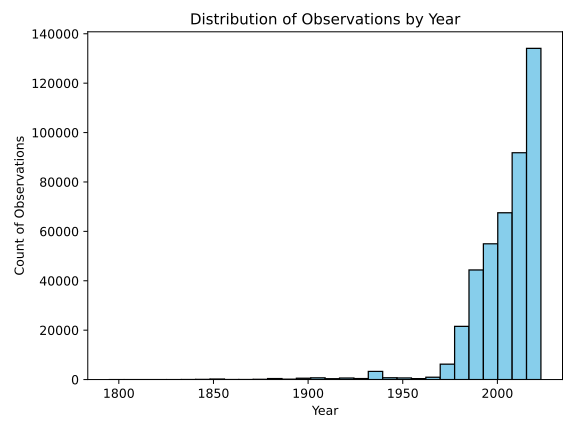
\includegraphics[width=0.6\linewidth]{figures/observation_distribution_by_year.png}
    \caption{Observations Distribution By Year}
\end{figure}

It is noticeable that the majority of the observations were registered over the 21st century and that the number of observations has been increasing over the past few decades. This could mean an increase in data accessibility and an improvement on fungus research and registration. Overall it seems to indicate good quality data as well as a tendency for more data to be available in the future.

\begin{figure}[H]
    \centering
    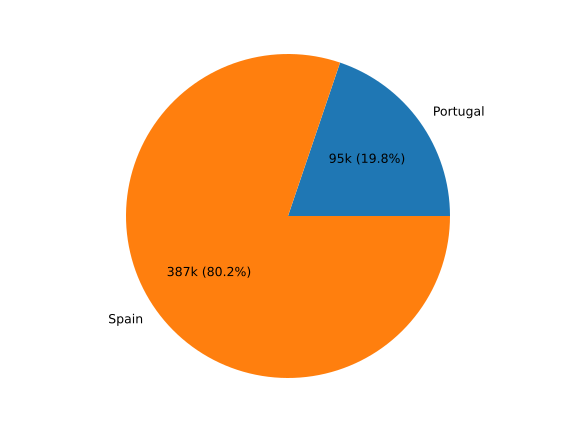
\includegraphics[width=0.6\linewidth]{figures/observation_distribution_by_country.png}
    \caption{Observations Count By Country}
\end{figure}

The number of registers available for Portugal and Spain seems to fairly represent the difference in area between these countries, so we conclude that the data adequately represents the diversity and characteristics of both countries, minimizing any potential bias.

\begin{figure}[H]
    \centering
    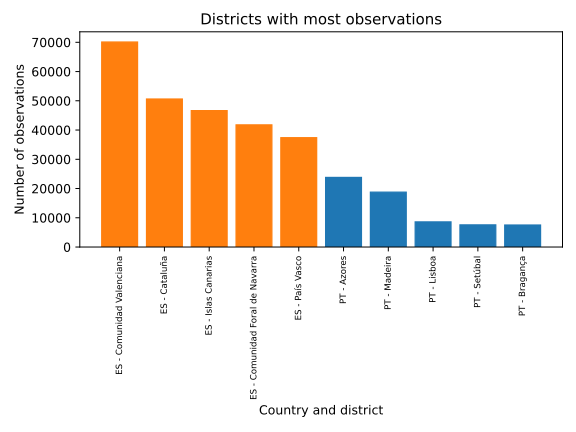
\includegraphics[width=0.6\linewidth]{figures/district_observations.png}
    \caption{Observations Distribution By District}
\end{figure}

As expected, the districts with most observations in Spain have a larger number of observations than the ones from Portugal. We can also observe that the archipelagos have the most observations from Portugal. 

\begin{figure}[H]
    \centering
    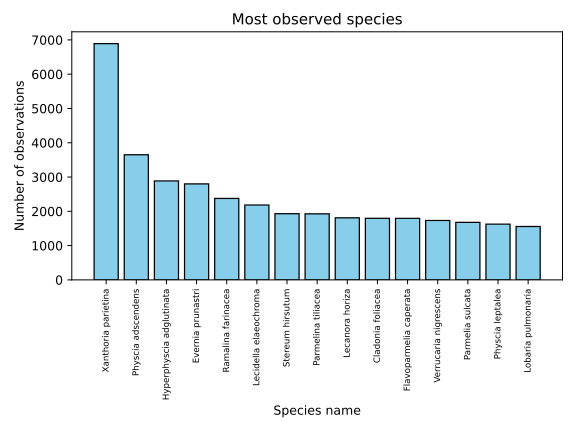
\includegraphics[width=0.6\linewidth]{figures/species_observations.png}
    \caption{Most Common Species}
\end{figure}

The 10 most frequent species' number of observations are all within the same order of magnitude.
